\chapter{Results}
\label{ch:testing}

\section{Simulation data}
In our testing we ran the simulation from 200 to over 1000 iterations, as there was no significant difference from 200 to 1000 iterations we did most of the simulations to 200 iterations.

The number of passengers was set to the ship maximum number of passengers stated on (website needed: http://www.cruisedeckplans.com/).

The hazards on-board the ship was set to increase at every second time step, both in number of nodes and how deadly it was in a particular node. In ACO, at each time step, the passengers was set to use 200 ants to find their way trough the ship, and each ant holding 200 pheromones to spread around. Also in each of these simulation, one fire was started, however some times it was randomly chosen one to three times.

In some of our simulation, it happens that a passenger would walk on board the ship for much longer then 300 time steps. However we have cut the graph at 300 time steps, as this would show more details in the graph about the algorithms and the average number of survives past 300 did not change.


\subsection{Celebrity Xpedition}

\begin{figure} [h]
\centering
\hspace*{-5.5in}
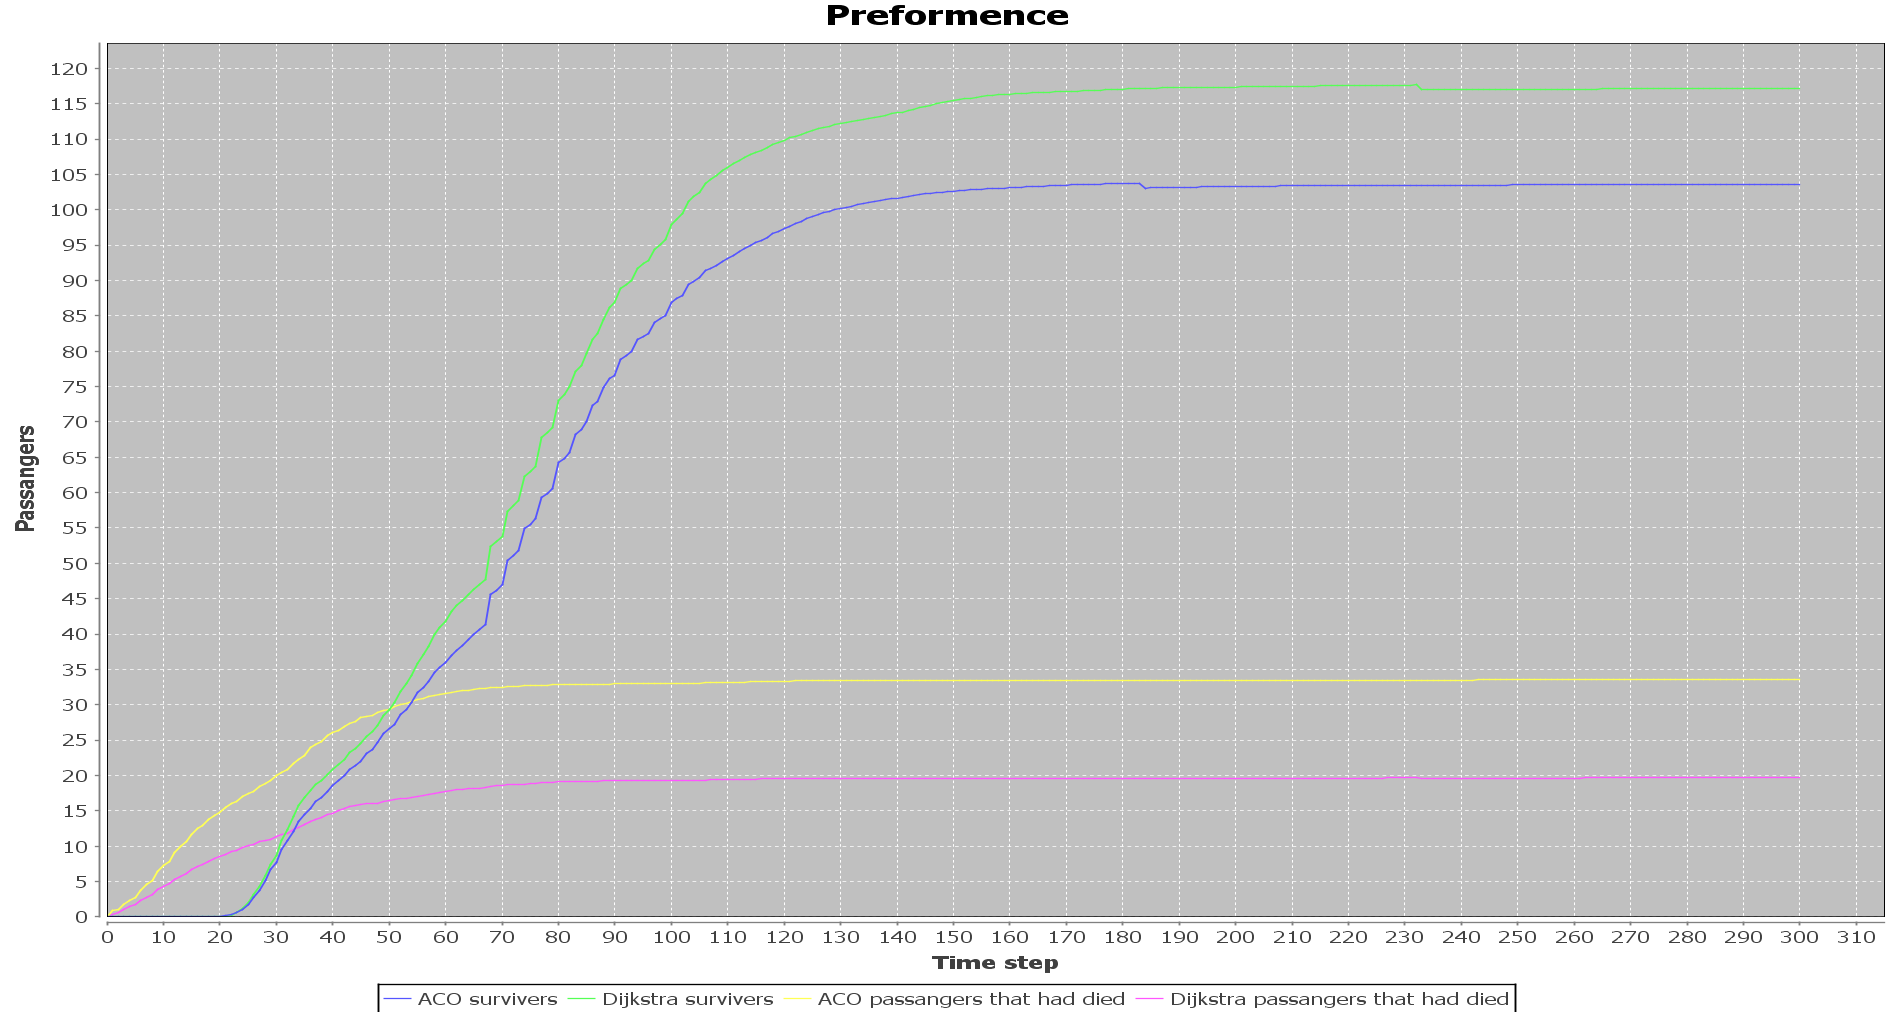
\includegraphics[scale=0.35]{images/Graph using 200 rounds 140 passangers and shortest first one hazzard.png}
\caption{The graph showing survives and deaths over a time table}
\label{fig:celebSafty}
\end{figure}

In this first chart you can see how well the different algorithms did. In both cases we only used one hazard(Fire) that spread on board the ship. As shown in the graph, Dijkstra outperforms ACO in both early and late stages of this graph. In the beginning there are more passengers dying to ACO chosen path then there is in Dijkstras choesen path, a good sign that both are finding different paths. As shortest path is measured in shortest time needed rather then shortest way to exit, it may be that Dijkstra spread the passangers more out then ACO.

Even when more passengers are dying at the beginning of the simulations, they both have the same boost in saved passengers at each time step.

The biggest problem for ACO over Dikstra is avoiding the hazards. Shown in the graph you can see that the death toll for ACO increases faster then Dijkstras death toll.

\begin{figure} [h]
\centering
\hspace*{-5.5in}
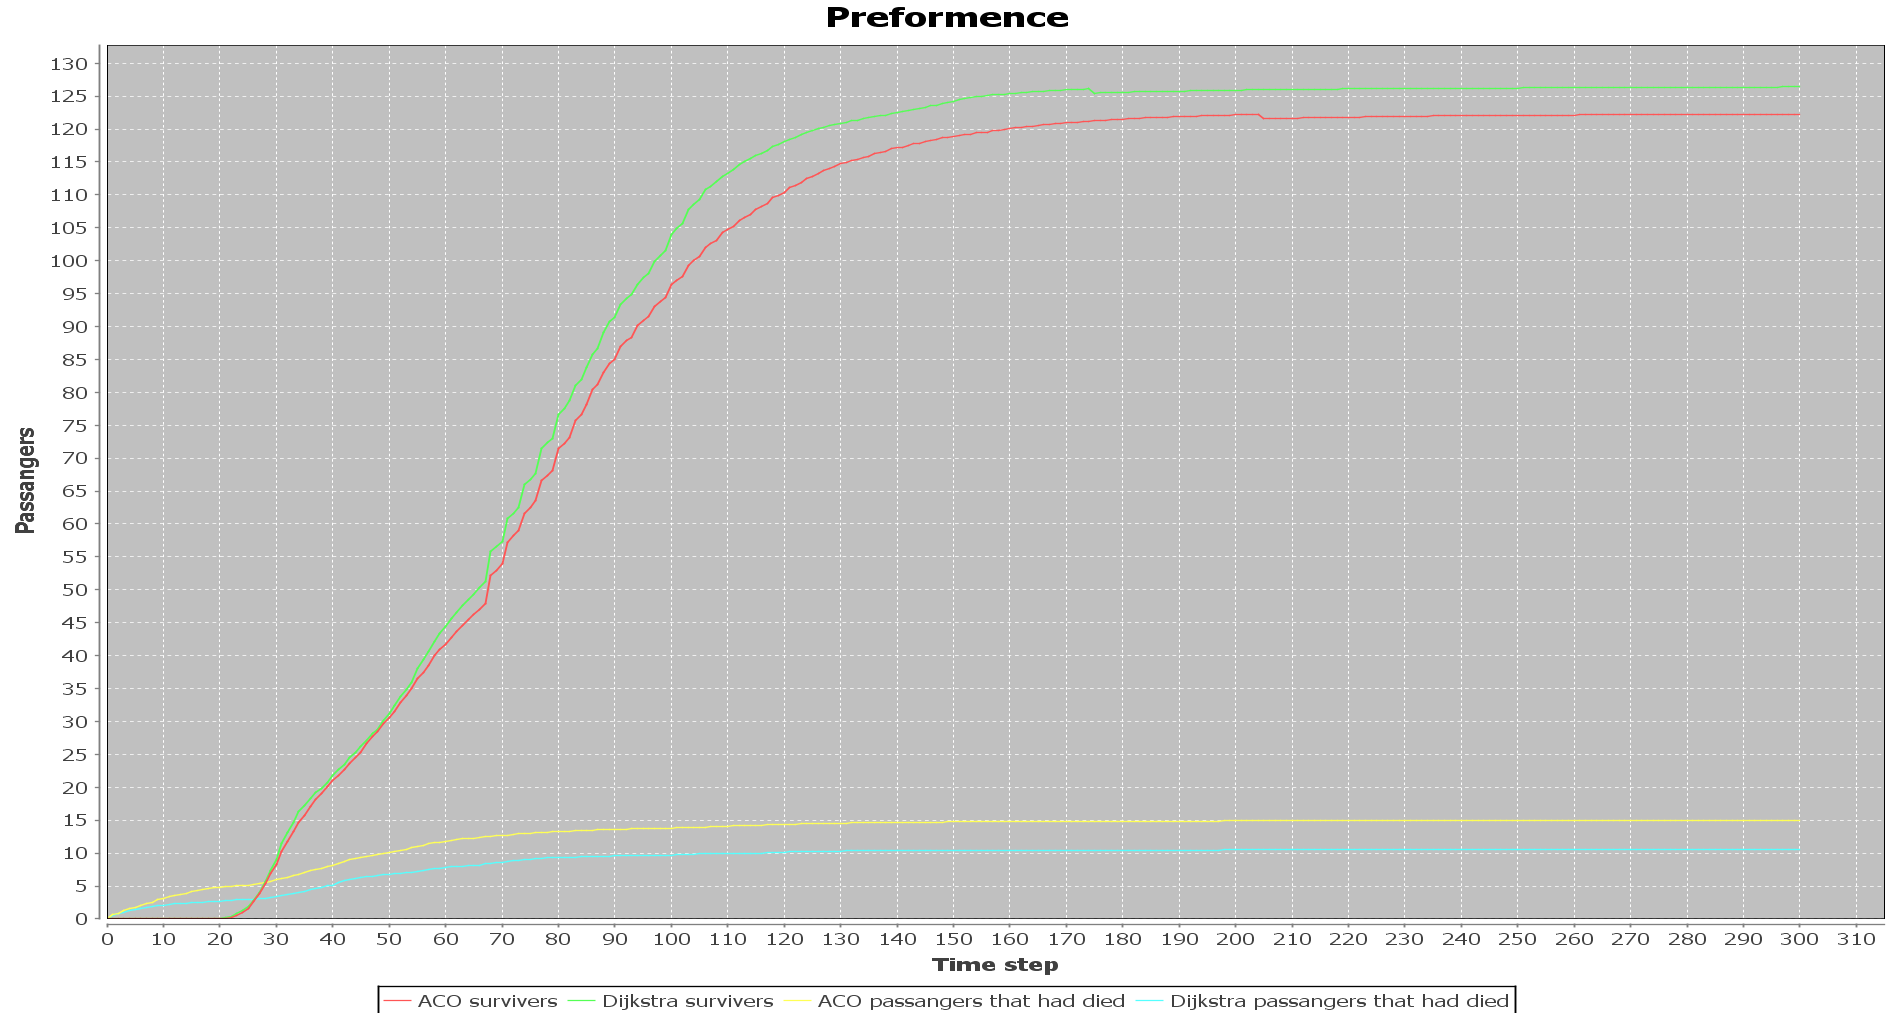
\includegraphics[scale=0.35]{images/Graph using 200 rounds 140 passangers and safest first one hazzard.png}
\caption{The graph showing survives and deaths over a time table}
\label{fig:celebSafty}
\end{figure}

In this second chart, we are using the same parameters as the first one, only difference is that we are looking after the safest path rather then the shortest path for the passengers. It is clearly shown that the death toll on the passengers is far lower then the previous one.
However Dijkstra proves yet again to outperform ACO in this instance. After about 30 time steps Dijkstra starts to pull ahead of ACO in number of passengers it have guided to the lifeboats. Even in number of deaths it is shown that Dijkstra is better at avoiding them.

If you look at Dijkstra in both cases, the number of deaths when looking after the safest path is 50\% less when looking for the shortest path.